\href{https://github.com/yassienE4/OS-VM/commit/3846ae8b48fa572486c9cc3fb142f36fbf4de522}{\ul{https://github.com/yassienE4/OS-VM/commit/3846ae8b48fa572486c9cc3fb142f36fbf4de522}}\\
How to run

\begin{enumerate}
\def\labelenumi{\arabic{enumi}.}
\item
  cd deadlock
\item
  change /input.txt (with ur input)
\item
  ./run.sh main.cpp
\end{enumerate}

I created a data structure called system state that stores the required
data

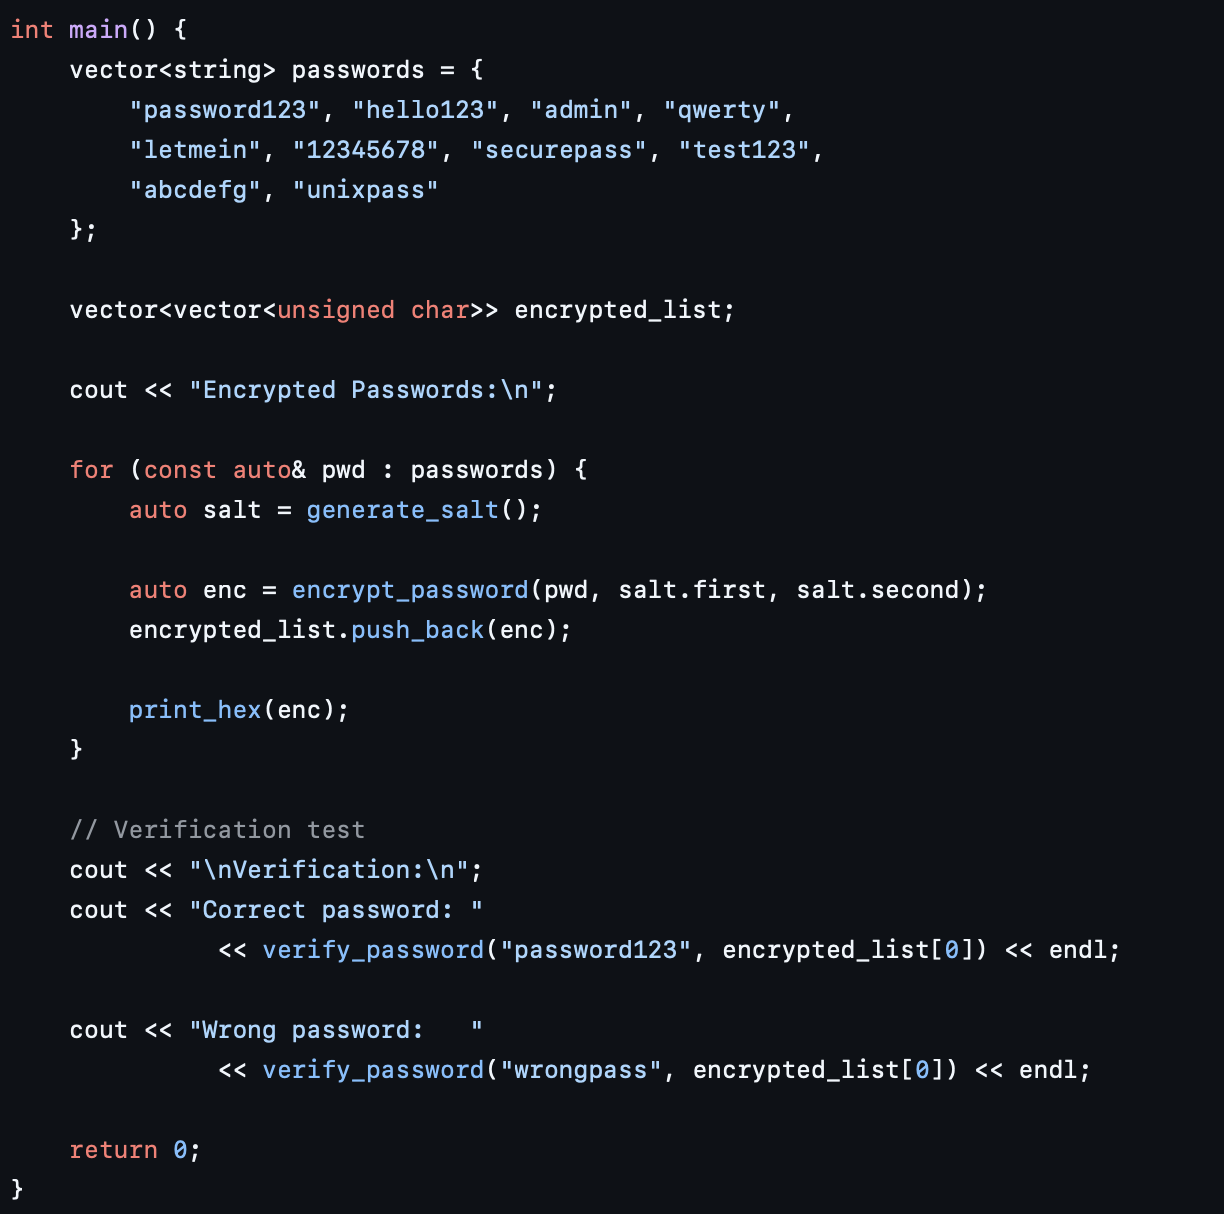
\includegraphics[width=6.5in,height=2.59722in]{./images/media/image3.png}

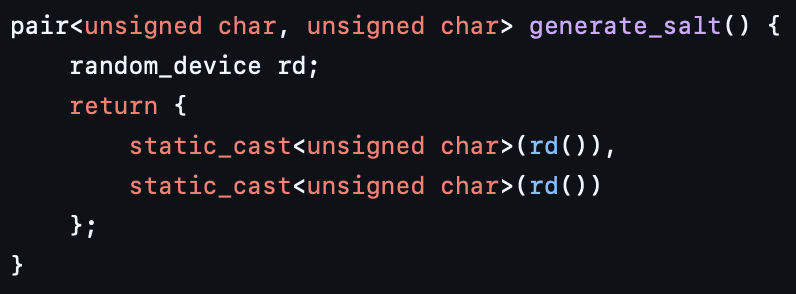
\includegraphics[width=6.5in,height=5.625in]{./images/media/image1.png}

This parses a txt file in this format

Example

\textbf{2 2}

\textbf{1 1}

\textbf{1 0}

\textbf{0 1}

\textbf{0 1}

\textbf{1 0}

Becomes

N = 2 (number of processes)

M = 2 (number of resource types)

E = {[}1,1{]}

C = {[}1 0{]} {[}0 1{]}

R = {[}0 1{]} {[}1 0{]}

The actual algorithm

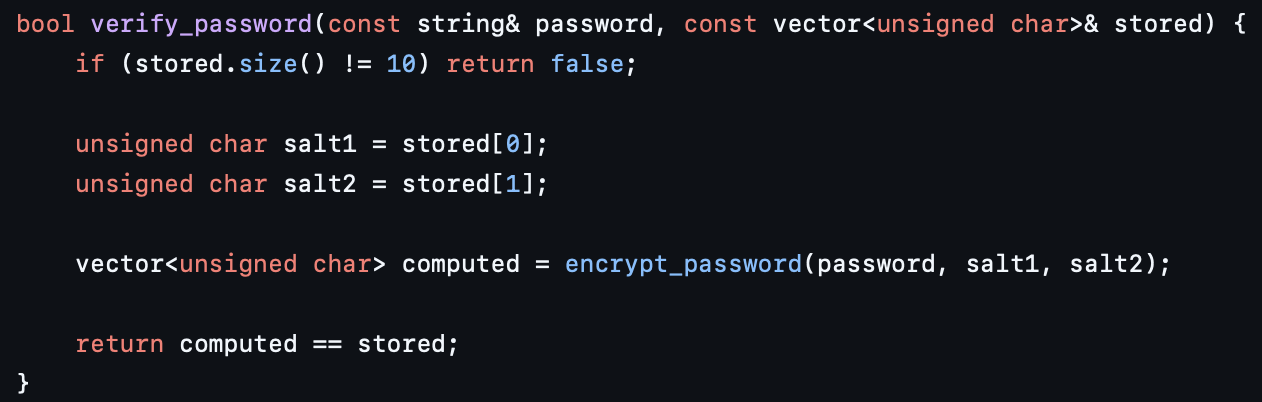
\includegraphics[width=2.83572in,height=7.94271in]{./images/media/image2.png}

The algorithm works by first computing the available resource vector. We
do this by subtracting the currently allocated resources for every
process and every resource type in a new vector called A.

We then create another vector, size n with default value false, used to
represent whether a process can eventually complete.

We then check for every process Pi that is not finished whether its
remaining request can be satisfied. We check that via the condition
R{[}i{]}{[}j{]} \textless= A{[}j{]} for all resource types j.

If the condition holds then the process can be completed.

If it runs, we simulate completion, release the allocation back to the
system and mark the process as finished, and also set progress = true.

If no process can run during a full iteration, progress becomes false
and the loop stops.

At this point the algorithm has determined the final state.

Finally we check if any processes remain unfinished.

if finished{[}i{]} == false

These processes are considered deadlocked, because none of them could
obtain the resources required to finish.
